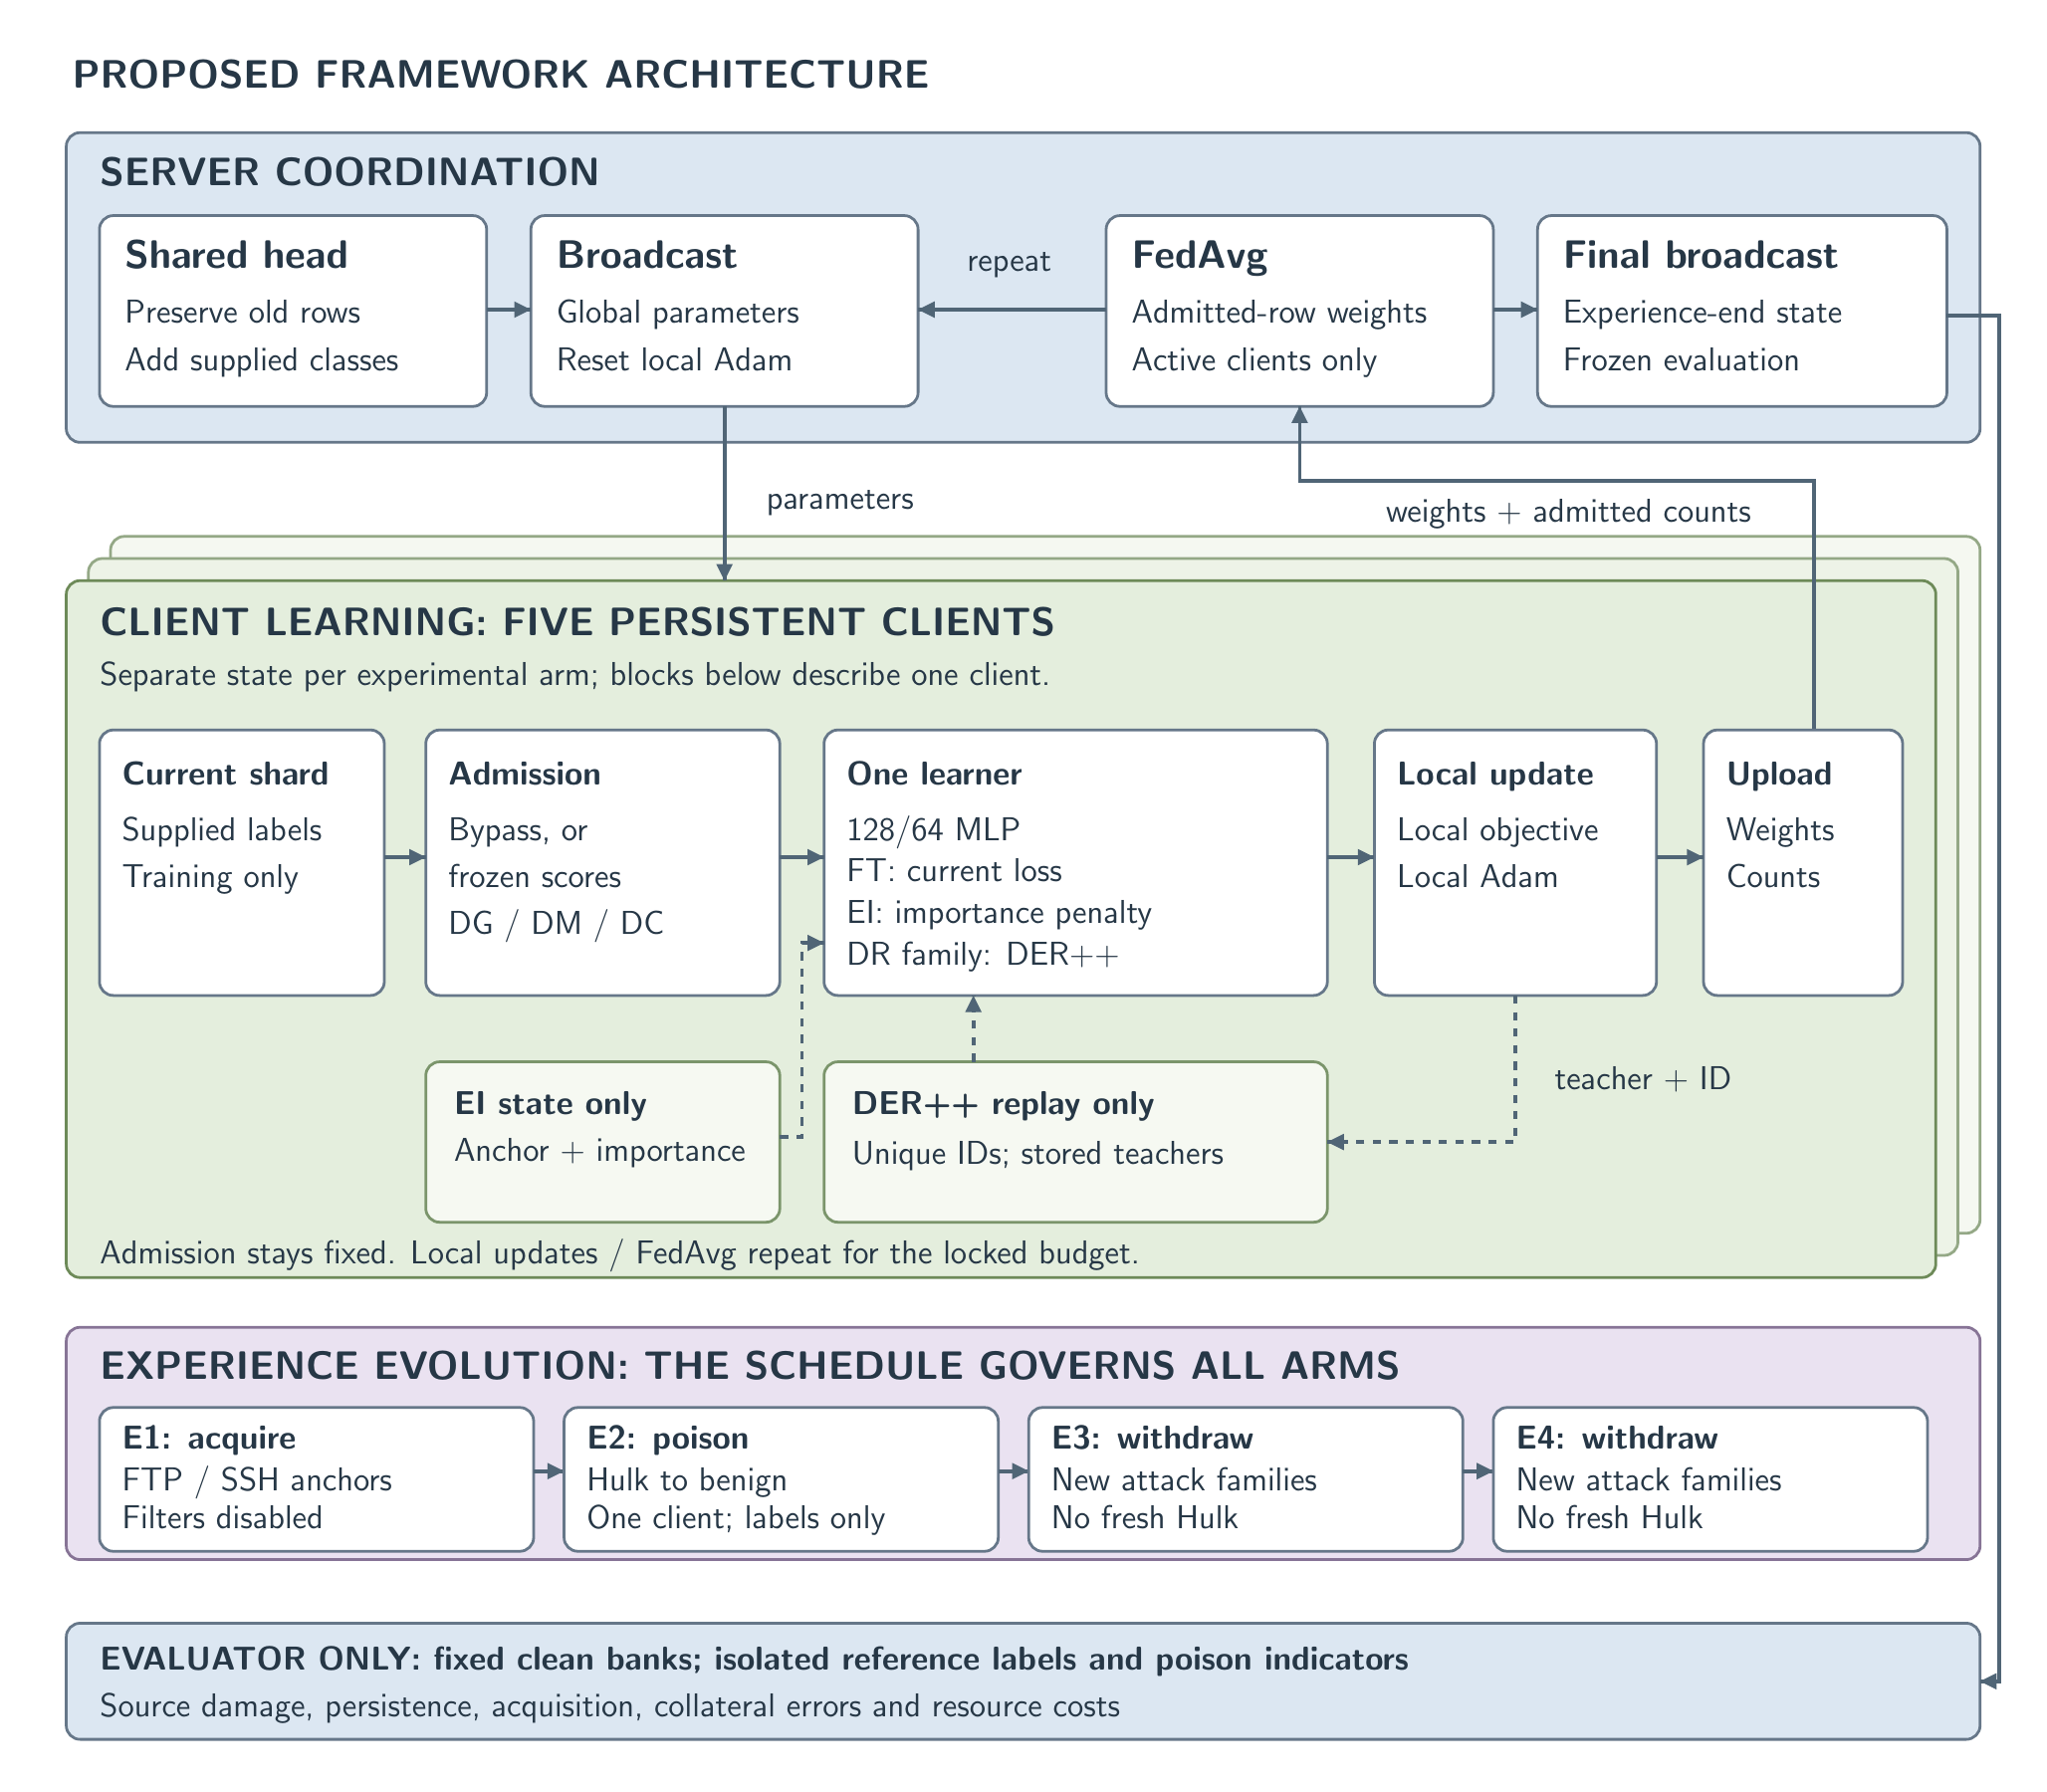
\begin{tikzpicture}[x=1bp,y=-1bp]
\path[use as bounding box] (0,0) rectangle (720,628);
\node[anchor=base west,inner sep=0,text={rgb,255:red,38;green,55;blue,70},font=\sffamily\bfseries\fontsize{15}{17.25}\selectfont] at (16,22) {PROPOSED FRAMEWORK ARCHITECTURE};
\path[draw={rgb,255:red,102;green,119;blue,137},fill={rgb,255:red,220;green,231;blue,242},line width=1bp,rounded corners=5bp] (14,38) rectangle (706,150);
\node[anchor=base west,inner sep=0,text={rgb,255:red,38;green,55;blue,70},font=\sffamily\bfseries\fontsize{15}{17.25}\selectfont] at (26,57) {SERVER COORDINATION};
\path[draw={rgb,255:red,102;green,119;blue,137},fill={rgb,255:red,255;green,255;blue,255},line width=1bp,rounded corners=5bp] (26,68) rectangle (166,137);
\node[anchor=base west,inner sep=0,text={rgb,255:red,38;green,55;blue,70},font=\sffamily\bfseries\fontsize{14}{16.099999999999998}\selectfont] at (35,87) {Shared head};
\node[anchor=base west,inner sep=0,text={rgb,255:red,38;green,55;blue,70},font=\sffamily\fontsize{12}{13.799999999999999}\selectfont] at (35,107) {Preserve old rows};
\node[anchor=base west,inner sep=0,text={rgb,255:red,38;green,55;blue,70},font=\sffamily\fontsize{12}{13.799999999999999}\selectfont] at (35,124) {Add supplied classes};
\path[draw={rgb,255:red,102;green,119;blue,137},fill={rgb,255:red,255;green,255;blue,255},line width=1bp,rounded corners=5bp] (182,68) rectangle (322,137);
\node[anchor=base west,inner sep=0,text={rgb,255:red,38;green,55;blue,70},font=\sffamily\bfseries\fontsize{14}{16.099999999999998}\selectfont] at (191,87) {Broadcast};
\node[anchor=base west,inner sep=0,text={rgb,255:red,38;green,55;blue,70},font=\sffamily\fontsize{12}{13.799999999999999}\selectfont] at (191,107) {Global parameters};
\node[anchor=base west,inner sep=0,text={rgb,255:red,38;green,55;blue,70},font=\sffamily\fontsize{12}{13.799999999999999}\selectfont] at (191,124) {Reset local Adam};
\path[draw={rgb,255:red,102;green,119;blue,137},fill={rgb,255:red,255;green,255;blue,255},line width=1bp,rounded corners=5bp] (390,68) rectangle (530,137);
\node[anchor=base west,inner sep=0,text={rgb,255:red,38;green,55;blue,70},font=\sffamily\bfseries\fontsize{14}{16.099999999999998}\selectfont] at (399,87) {FedAvg};
\node[anchor=base west,inner sep=0,text={rgb,255:red,38;green,55;blue,70},font=\sffamily\fontsize{12}{13.799999999999999}\selectfont] at (399,107) {Admitted-row weights};
\node[anchor=base west,inner sep=0,text={rgb,255:red,38;green,55;blue,70},font=\sffamily\fontsize{12}{13.799999999999999}\selectfont] at (399,124) {Active clients only};
\path[draw={rgb,255:red,102;green,119;blue,137},fill={rgb,255:red,255;green,255;blue,255},line width=1bp,rounded corners=5bp] (546,68) rectangle (694,137);
\node[anchor=base west,inner sep=0,text={rgb,255:red,38;green,55;blue,70},font=\sffamily\bfseries\fontsize{14}{16.099999999999998}\selectfont] at (555,87) {Final broadcast};
\node[anchor=base west,inner sep=0,text={rgb,255:red,38;green,55;blue,70},font=\sffamily\fontsize{12}{13.799999999999999}\selectfont] at (555,107) {Experience-end state};
\node[anchor=base west,inner sep=0,text={rgb,255:red,38;green,55;blue,70},font=\sffamily\fontsize{12}{13.799999999999999}\selectfont] at (555,124) {Frozen evaluation};
\path[draw={rgb,255:red,80;green,101;blue,118},line width=1.4bp] (166,102) -- (182,102);
\path[fill={rgb,255:red,80;green,101;blue,118}] (182.000,102.000) -- (176.000,99.000) -- (176.000,105.000) -- cycle;
\path[draw={rgb,255:red,80;green,101;blue,118},line width=1.4bp] (530,102) -- (546,102);
\path[fill={rgb,255:red,80;green,101;blue,118}] (546.000,102.000) -- (540.000,99.000) -- (540.000,105.000) -- cycle;
\path[draw={rgb,255:red,80;green,101;blue,118},line width=1.4bp] (390,102) -- (322,102);
\path[fill={rgb,255:red,80;green,101;blue,118}] (322.000,102.000) -- (328.000,105.000) -- (328.000,99.000) -- cycle;
\node[anchor=base,inner sep=0,text={rgb,255:red,38;green,55;blue,70},font=\sffamily\fontsize{12}{13.799999999999999}\selectfont] at (355,88) {repeat};
\path[draw={rgb,255:red,148;green,168;blue,134},fill={rgb,255:red,245;green,248;blue,241},line width=1bp,rounded corners=5bp] (30,184) rectangle (706,436);
\path[draw={rgb,255:red,148;green,168;blue,134},fill={rgb,255:red,237;green,243;blue,231},line width=1bp,rounded corners=5bp] (22,192) rectangle (698,444);
\path[draw={rgb,255:red,109;green,138;blue,88},fill={rgb,255:red,228;green,238;blue,221},line width=1bp,rounded corners=5bp] (14,200) rectangle (690,452);
\node[anchor=base west,inner sep=0,text={rgb,255:red,38;green,55;blue,70},font=\sffamily\bfseries\fontsize{15}{17.25}\selectfont] at (26,220) {CLIENT LEARNING: FIVE PERSISTENT CLIENTS};
\node[anchor=base west,inner sep=0,text={rgb,255:red,38;green,55;blue,70},font=\sffamily\fontsize{12}{13.799999999999999}\selectfont] at (26,238) {Separate state per experimental arm; blocks below describe one client.};
\path[draw={rgb,255:red,80;green,101;blue,118},line width=1.4bp] (252,137) -- (252,200);
\path[fill={rgb,255:red,80;green,101;blue,118}] (252.000,200.000) -- (255.000,194.000) -- (249.000,194.000) -- cycle;
\node[anchor=base west,inner sep=0,text={rgb,255:red,38;green,55;blue,70},font=\sffamily\fontsize{12}{13.799999999999999}\selectfont] at (267,174) {parameters};
\path[draw={rgb,255:red,80;green,101;blue,118},line width=1.4bp] (646,254) -- (646,164) -- (460,164) -- (460,137);
\path[fill={rgb,255:red,80;green,101;blue,118}] (460.000,137.000) -- (457.000,143.000) -- (463.000,143.000) -- cycle;
\node[anchor=base west,inner sep=0,text={rgb,255:red,38;green,55;blue,70},font=\sffamily\fontsize{12}{13.799999999999999}\selectfont] at (491,179) {weights + admitted counts};
\path[draw={rgb,255:red,102;green,119;blue,137},fill={rgb,255:red,255;green,255;blue,255},line width=1bp,rounded corners=5bp] (26,254) rectangle (129,350);
\node[anchor=base west,inner sep=0,text={rgb,255:red,38;green,55;blue,70},font=\sffamily\bfseries\fontsize{13}{14.95}\selectfont] at (34,274) {Current shard};
\node[anchor=base west,inner sep=0,text={rgb,255:red,38;green,55;blue,70},font=\sffamily\fontsize{12}{13.799999999999999}\selectfont] at (34,294) {Supplied labels};
\node[anchor=base west,inner sep=0,text={rgb,255:red,38;green,55;blue,70},font=\sffamily\fontsize{12}{13.799999999999999}\selectfont] at (34,311) {Training only};
\path[draw={rgb,255:red,102;green,119;blue,137},fill={rgb,255:red,255;green,255;blue,255},line width=1bp,rounded corners=5bp] (144,254) rectangle (272,350);
\node[anchor=base west,inner sep=0,text={rgb,255:red,38;green,55;blue,70},font=\sffamily\bfseries\fontsize{13}{14.95}\selectfont] at (152,274) {Admission};
\node[anchor=base west,inner sep=0,text={rgb,255:red,38;green,55;blue,70},font=\sffamily\fontsize{12}{13.799999999999999}\selectfont] at (152,294) {Bypass, or};
\node[anchor=base west,inner sep=0,text={rgb,255:red,38;green,55;blue,70},font=\sffamily\fontsize{12}{13.799999999999999}\selectfont] at (152,311) {frozen scores};
\node[anchor=base west,inner sep=0,text={rgb,255:red,38;green,55;blue,70},font=\sffamily\fontsize{12}{13.799999999999999}\selectfont] at (152,328) {DG / DM / DC};
\path[draw={rgb,255:red,102;green,119;blue,137},fill={rgb,255:red,255;green,255;blue,255},line width=1bp,rounded corners=5bp] (288,254) rectangle (470,350);
\node[anchor=base west,inner sep=0,text={rgb,255:red,38;green,55;blue,70},font=\sffamily\bfseries\fontsize{13}{14.95}\selectfont] at (296,274) {One learner};
\node[anchor=base west,inner sep=0,text={rgb,255:red,38;green,55;blue,70},font=\sffamily\fontsize{12}{13.799999999999999}\selectfont] at (296,294) {128/64 MLP};
\node[anchor=base west,inner sep=0,text={rgb,255:red,38;green,55;blue,70},font=\sffamily\fontsize{12}{13.799999999999999}\selectfont] at (296,309) {FT: current loss};
\node[anchor=base west,inner sep=0,text={rgb,255:red,38;green,55;blue,70},font=\sffamily\fontsize{12}{13.799999999999999}\selectfont] at (296,324) {EI: importance penalty};
\node[anchor=base west,inner sep=0,text={rgb,255:red,38;green,55;blue,70},font=\sffamily\fontsize{12}{13.799999999999999}\selectfont] at (296,339) {DR family: DER++};
\path[draw={rgb,255:red,102;green,119;blue,137},fill={rgb,255:red,255;green,255;blue,255},line width=1bp,rounded corners=5bp] (487,254) rectangle (589,350);
\node[anchor=base west,inner sep=0,text={rgb,255:red,38;green,55;blue,70},font=\sffamily\bfseries\fontsize{13}{14.95}\selectfont] at (495,274) {Local update};
\node[anchor=base west,inner sep=0,text={rgb,255:red,38;green,55;blue,70},font=\sffamily\fontsize{12}{13.799999999999999}\selectfont] at (495,294) {Local objective};
\node[anchor=base west,inner sep=0,text={rgb,255:red,38;green,55;blue,70},font=\sffamily\fontsize{12}{13.799999999999999}\selectfont] at (495,311) {Local Adam};
\path[draw={rgb,255:red,102;green,119;blue,137},fill={rgb,255:red,255;green,255;blue,255},line width=1bp,rounded corners=5bp] (606,254) rectangle (678,350);
\node[anchor=base west,inner sep=0,text={rgb,255:red,38;green,55;blue,70},font=\sffamily\bfseries\fontsize{13}{14.95}\selectfont] at (614,274) {Upload};
\node[anchor=base west,inner sep=0,text={rgb,255:red,38;green,55;blue,70},font=\sffamily\fontsize{12}{13.799999999999999}\selectfont] at (614,294) {Weights};
\node[anchor=base west,inner sep=0,text={rgb,255:red,38;green,55;blue,70},font=\sffamily\fontsize{12}{13.799999999999999}\selectfont] at (614,311) {Counts};
\path[draw={rgb,255:red,80;green,101;blue,118},line width=1.4bp] (129,300) -- (144,300);
\path[fill={rgb,255:red,80;green,101;blue,118}] (144.000,300.000) -- (138.000,297.000) -- (138.000,303.000) -- cycle;
\path[draw={rgb,255:red,80;green,101;blue,118},line width=1.4bp] (272,300) -- (288,300);
\path[fill={rgb,255:red,80;green,101;blue,118}] (288.000,300.000) -- (282.000,297.000) -- (282.000,303.000) -- cycle;
\path[draw={rgb,255:red,80;green,101;blue,118},line width=1.4bp] (470,300) -- (487,300);
\path[fill={rgb,255:red,80;green,101;blue,118}] (487.000,300.000) -- (481.000,297.000) -- (481.000,303.000) -- cycle;
\path[draw={rgb,255:red,80;green,101;blue,118},line width=1.4bp] (589,300) -- (606,300);
\path[fill={rgb,255:red,80;green,101;blue,118}] (606.000,300.000) -- (600.000,297.000) -- (600.000,303.000) -- cycle;
\path[draw={rgb,255:red,123;green,149;blue,107},fill={rgb,255:red,246;green,249;blue,242},line width=1bp,rounded corners=5bp] (144,374) rectangle (272,432);
\node[anchor=base west,inner sep=0,text={rgb,255:red,38;green,55;blue,70},font=\sffamily\bfseries\fontsize{13}{14.95}\selectfont] at (154,393) {EI state only};
\node[anchor=base west,inner sep=0,text={rgb,255:red,38;green,55;blue,70},font=\sffamily\fontsize{12}{13.799999999999999}\selectfont] at (154,410) {Anchor + importance};
\path[draw={rgb,255:red,80;green,101;blue,118},line width=1.4bp,dashed] (272,401) -- (280,401) -- (280,331) -- (288,331);
\path[fill={rgb,255:red,80;green,101;blue,118}] (288.000,331.000) -- (282.000,328.000) -- (282.000,334.000) -- cycle;
\path[draw={rgb,255:red,123;green,149;blue,107},fill={rgb,255:red,246;green,249;blue,242},line width=1bp,rounded corners=5bp] (288,374) rectangle (470,432);
\node[anchor=base west,inner sep=0,text={rgb,255:red,38;green,55;blue,70},font=\sffamily\bfseries\fontsize{13}{14.95}\selectfont] at (298,393) {DER++ replay only};
\node[anchor=base west,inner sep=0,text={rgb,255:red,38;green,55;blue,70},font=\sffamily\fontsize{12}{13.799999999999999}\selectfont] at (298,411) {Unique IDs; stored teachers};
\path[draw={rgb,255:red,80;green,101;blue,118},line width=1.4bp,dashed] (342,374) -- (342,350);
\path[fill={rgb,255:red,80;green,101;blue,118}] (342.000,350.000) -- (339.000,356.000) -- (345.000,356.000) -- cycle;
\path[draw={rgb,255:red,80;green,101;blue,118},line width=1.4bp,dashed] (538,350) -- (538,403) -- (470,403);
\path[fill={rgb,255:red,80;green,101;blue,118}] (470.000,403.000) -- (476.000,406.000) -- (476.000,400.000) -- cycle;
\node[anchor=base west,inner sep=0,text={rgb,255:red,38;green,55;blue,70},font=\sffamily\fontsize{12}{13.799999999999999}\selectfont] at (552,384) {teacher + ID};
\node[anchor=base west,inner sep=0,text={rgb,255:red,38;green,55;blue,70},font=\sffamily\fontsize{12}{13.799999999999999}\selectfont] at (26,447) {Admission stays fixed. Local updates / FedAvg repeat for the locked budget.};
\path[draw={rgb,255:red,135;green,116;blue,150},fill={rgb,255:red,234;green,226;blue,241},line width=1bp,rounded corners=5bp] (14,470) rectangle (706,554);
\node[anchor=base west,inner sep=0,text={rgb,255:red,38;green,55;blue,70},font=\sffamily\bfseries\fontsize{15}{17.25}\selectfont] at (26,489) {EXPERIENCE EVOLUTION: THE SCHEDULE GOVERNS ALL ARMS};
\path[draw={rgb,255:red,102;green,119;blue,137},fill={rgb,255:red,255;green,255;blue,255},line width=1bp,rounded corners=5bp] (26,499) rectangle (183,551);
\node[anchor=base west,inner sep=0,text={rgb,255:red,38;green,55;blue,70},font=\sffamily\bfseries\fontsize{13}{14.95}\selectfont] at (34,514) {E1: acquire};
\node[anchor=base west,inner sep=0,text={rgb,255:red,38;green,55;blue,70},font=\sffamily\fontsize{12}{13.799999999999999}\selectfont] at (34,529) {FTP / SSH anchors};
\node[anchor=base west,inner sep=0,text={rgb,255:red,38;green,55;blue,70},font=\sffamily\fontsize{12}{13.799999999999999}\selectfont] at (34,543) {Filters disabled};
\path[draw={rgb,255:red,80;green,101;blue,118},line width=1.4bp] (183,522) -- (194,522);
\path[fill={rgb,255:red,80;green,101;blue,118}] (194.000,522.000) -- (188.000,519.000) -- (188.000,525.000) -- cycle;
\path[draw={rgb,255:red,102;green,119;blue,137},fill={rgb,255:red,255;green,255;blue,255},line width=1bp,rounded corners=5bp] (194,499) rectangle (351,551);
\node[anchor=base west,inner sep=0,text={rgb,255:red,38;green,55;blue,70},font=\sffamily\bfseries\fontsize{13}{14.95}\selectfont] at (202,514) {E2: poison};
\node[anchor=base west,inner sep=0,text={rgb,255:red,38;green,55;blue,70},font=\sffamily\fontsize{12}{13.799999999999999}\selectfont] at (202,529) {Hulk to benign};
\node[anchor=base west,inner sep=0,text={rgb,255:red,38;green,55;blue,70},font=\sffamily\fontsize{12}{13.799999999999999}\selectfont] at (202,543) {One client; labels only};
\path[draw={rgb,255:red,80;green,101;blue,118},line width=1.4bp] (351,522) -- (362,522);
\path[fill={rgb,255:red,80;green,101;blue,118}] (362.000,522.000) -- (356.000,519.000) -- (356.000,525.000) -- cycle;
\path[draw={rgb,255:red,102;green,119;blue,137},fill={rgb,255:red,255;green,255;blue,255},line width=1bp,rounded corners=5bp] (362,499) rectangle (519,551);
\node[anchor=base west,inner sep=0,text={rgb,255:red,38;green,55;blue,70},font=\sffamily\bfseries\fontsize{13}{14.95}\selectfont] at (370,514) {E3: withdraw};
\node[anchor=base west,inner sep=0,text={rgb,255:red,38;green,55;blue,70},font=\sffamily\fontsize{12}{13.799999999999999}\selectfont] at (370,529) {New attack families};
\node[anchor=base west,inner sep=0,text={rgb,255:red,38;green,55;blue,70},font=\sffamily\fontsize{12}{13.799999999999999}\selectfont] at (370,543) {No fresh Hulk};
\path[draw={rgb,255:red,80;green,101;blue,118},line width=1.4bp] (519,522) -- (530,522);
\path[fill={rgb,255:red,80;green,101;blue,118}] (530.000,522.000) -- (524.000,519.000) -- (524.000,525.000) -- cycle;
\path[draw={rgb,255:red,102;green,119;blue,137},fill={rgb,255:red,255;green,255;blue,255},line width=1bp,rounded corners=5bp] (530,499) rectangle (687,551);
\node[anchor=base west,inner sep=0,text={rgb,255:red,38;green,55;blue,70},font=\sffamily\bfseries\fontsize{13}{14.95}\selectfont] at (538,514) {E4: withdraw};
\node[anchor=base west,inner sep=0,text={rgb,255:red,38;green,55;blue,70},font=\sffamily\fontsize{12}{13.799999999999999}\selectfont] at (538,529) {New attack families};
\node[anchor=base west,inner sep=0,text={rgb,255:red,38;green,55;blue,70},font=\sffamily\fontsize{12}{13.799999999999999}\selectfont] at (538,543) {No fresh Hulk};
\path[draw={rgb,255:red,102;green,119;blue,137},fill={rgb,255:red,220;green,231;blue,242},line width=1bp,rounded corners=5bp] (14,577) rectangle (706,619);
\node[anchor=base west,inner sep=0,text={rgb,255:red,38;green,55;blue,70},font=\sffamily\bfseries\fontsize{13}{14.95}\selectfont] at (26,594) {EVALUATOR ONLY: fixed clean banks; isolated reference labels and poison indicators};
\node[anchor=base west,inner sep=0,text={rgb,255:red,38;green,55;blue,70},font=\sffamily\fontsize{12}{13.799999999999999}\selectfont] at (26,611) {Source damage, persistence, acquisition, collateral errors and resource costs};
\path[draw={rgb,255:red,80;green,101;blue,118},line width=1.4bp] (694,104) -- (713,104) -- (713,598) -- (706,598);
\path[fill={rgb,255:red,80;green,101;blue,118}] (706.000,598.000) -- (712.000,601.000) -- (712.000,595.000) -- cycle;
\end{tikzpicture}